\section{The second and third tracks}
\label{app:tracks}

Both tracks keep the first track's protocol. Tasks return with fresh instances after gaps while new tasks keep arriving, the learner may ask for a demonstration or act, a failure costs the whole budget, and after the stream the learner is frozen and plays a seen test and a held-out test, each read against the learner wiped before every instance. Each is its edition's configuration in the released code (\texttt{v0.6.0}), at seed 0. Since users bring tasks of their own, the second track's pool serves at most four users and the third's one. A verified run on either track plays a private set of its own, 50 new rules on ARC-AGI-2 and 25 new games on ARC-AGI-3 (Appendix~\ref{app:heldout}).

\paragraph{ARC-AGI-2.} Of ARC-AGI-2's 1,000 public training tasks, 767 are ARC-AGI-1 tasks, as are 6 of its 120 evaluation tasks \citep{chollet2025arcagi2}, so the track draws only on tasks new to the second edition. ARC-GEN \citep{moffitt2025arcgen} has generators for 172 of the 233 new training tasks, and a task enters the pool when its generator passes a screen over 1,000 draws, the private set's mechanical filters (Appendix~\ref{app:heldout}) and two checks of fidelity. ARC-TGI \citep{lehmann2026arctgi} also offers generators for part of ARC-AGI-2, but the track uses ARC-GEN alone. ARC-GEN's own validation must reproduce every published pair, and every draw must keep what all the published pairs share, such as the output's shape, its scale and colors drawn from the input; the thresholds are in the track's code. Of the 172, 117 pass. The track streams 25 of them, eight fresh instances each, in the first track's order, and its held-out test is 100 of the 114 evaluation tasks new to ARC-AGI-2, each served with its own pairs. A demonstration is a fresh generated pair, as on the first track. The stream's tasks are training tasks, which, unlike the evaluation tasks, were not calibrated on people \citep{chollet2025arcagi2}, so the stream may be the easier half.

\paragraph{ARC-AGI-3.} Each of ARC-AGI-3's 25 public games is a 64 by 64 grid that responds to seven actions and a reset over a fixed sequence of levels \citep{arcprize2026arcagi3}. In 22 of the games the later levels add sprite types, and in several they change a rule's parameters, so a game's levels are not instances of one task. A task of the track is therefore a game's rules at its first level, and an instance a fresh level of those rules, with the same sprite types and data in a new layout. A generator we wrote for each game draws the level, and the game's solver, a search over the game's state, solves it and checks the answer by replaying it in ARC Prize's engine. A game enters the track only if its generator passes a gate over 50 seeds, which checks that every level is drawn quickly, solved and won on replay, close in length to the game's own first level, distinct from the others and from the public first level, and made of the first level's sprite types alone, with the thresholds in the track's code. All 25 games pass, and they are split once, at seed 0, into 15 that the stream serves and 10 held out. The track serves eight fresh levels of each stream game in the first track's order, its seen test four fresh levels of each, and its held-out test four of each held-out game.

An instance's baseline is the human count of actions for the game's first level, scaled by the instance's solution length over the first level's. Its budget of actions is five times its baseline, at most 1,000, and every action and every reset of the level counts toward it. A solved level costs its actions and resets over its baseline, at most 5, and one more for each demonstration, at most three; an unsolved level costs the whole budget of 8, so that failing is never cheaper than trying, as on the first track. A demonstration is the solver's play of another fresh level of the same game. Since no instance is a level anyone has played before, a memory of the public levels, with which a harness has solved that set \citep{bedi2026learningmachines}, as have three concurrent ones \citep{wu2026kepler,zhao2026memento3,anonymous2026comate}, does not help. Compiled Worlds \citep{anonymous2026compiledworlds}, also concurrent, edits the public games' programs into variants, resampled layouts and mutated rules among them, and prices what each change adds to a harness's cost on the original level. A game's later levels, with their new rules, are left for a mode of the benchmark in which the rules drift.

\paragraph{First sight.} Table~\ref{tab:first-sight} gives how often three models solve each track's instances at first sight. On ARC-AGI-2 a model sees three demonstrations and answers once, as the private set's calibration does (Appendix~\ref{app:heldout}). On ARC-AGI-3 it plays the held-out test, four fresh levels of each held-out game, wiped before each and free to ask for up to three demonstrations per level. Qwen3.5-9B's replies reached their cap before an answer on 61 of its 100 ARC-AGI-2 instances, and a provider's error ended 7 more, so its rate mostly counts replies cut off, as on the first track. On ARC-AGI-3, where a level takes tens to hundreds of moves, a quarter of its replies reasoned to the cap, some for over 20 minutes, and after two and a half hours it had made 30 of its first level's 110 moves, so we report no result there.

\paragraph{Kimi K3.1 Pro on ARC-AGI-2.} Kimi K3.1 Pro has no published ARC-AGI-2 score, but its 15\% or so on our held-out test, which serves 100 of ARC-AGI-2's own evaluation tasks with their own pairs, is in line with ARC Prize's results for Kimi K3 at low reasoning effort on the same tasks, 16 solved against 45 at high effort and 55 at max \citep{arcprize2026leaderboard}. Kimi offers only low, high and max effort, and at the medium we requested through OpenRouter its first-sight replies ran about 1,000 tokens at the median, a fifth of Kimi-K3's at the same setting, with none reaching the cap; played again on 50 of those instances on Moonshot AI's own endpoint, which served all our Kimi runs, medium solved 19 and 24 at replies as long as low's, which solved 23, against 40 and 44 at high, so our runs, which request medium, play Kimi at what is in effect its low effort. Its higher rates elsewhere come from easier tasks: ARC-AGI-2's training tasks in the stream and the seen test, which were not calibrated on people, and each ARC-AGI-3 game's first level, which ARC Prize designed to be easy \citep{arcprize2026arcagi3}, and nearly every level Kimi solved there it solved after watching the solver play another level of the same game.

\begin{table}[h]
\centering
\small
\caption{First-sight solve rates on the second and third tracks, in percent, with the number of instances, requested at medium reasoning effort through OpenRouter, a level Kimi does not offer. ARC-AGI-2: four fresh instances of each of the track's 25 stream tasks (two of each for Kimi-K3), three demonstrations and one answer, an exact match, a reply capped at 32{,}000 tokens, which no reply of the Kimi models reached, and at 65{,}536 for Qwen3.5-9B. ARC-AGI-3: the track's 40 held-out levels, the bare model wiped before each, a reply capped at 64{,}000 tokens, and the mean charge out of 8. A dash marks a track a model is too slow to play.}
\label{tab:first-sight}
\begin{tabular}{lrrrr}
\toprule
& \multicolumn{2}{c}{ARC-AGI-2} & \multicolumn{2}{c}{ARC-AGI-3} \\
\cmidrule(lr){2-3} \cmidrule(lr){4-5}
model & solved & instances & solved & mean charge \\
\midrule
Kimi K3.1 Pro & 29 & 100 & 25 & 6.8 \\
Kimi-K3 & 56 & 50 & 35 & 6.0 \\
Qwen3.5-9B & 22 & 100 & -- & -- \\
\bottomrule
\end{tabular}
\end{table}

\begin{table}[h]
\centering
\footnotesize\setlength{\tabcolsep}{3pt}
\caption{Initial results on the second and third tracks: Kimi K3.1 Pro, requested at medium reasoning effort, at one user, the two floors through OpenRouter and every other method pinned to Moonshot AI's own endpoint. $P$ is the share of the stream's instances solved, in percent. $L$, $S_{\mathrm{seen}}$ and $S_{\mathrm{held}}$ are read as in Table~\ref{tab:tests}, the demo-cache floor against the stateless floor, KA against K\textsubscript{0} and every other method against itself wiped, from four plays of each test by each floor and two by every other method, a method that keeps nothing reading half its plays against the other half. A dash marks a method that does not play ARC-AGI-3 beyond the pilot of Table~\ref{tab:arc3-pilot}. Small type is the 95\% interval over task resamples. Bold marks each column's best, for $L$ and $S$ among the values whose 95\% interval lies above zero.}
\label{tab:tracks-light}
\begin{adjustbox}{max width=\linewidth}
\begin{tabular}{lrr@{\hspace{0.3em}}lr@{\hspace{0.3em}}lr@{\hspace{0.3em}}l@{\hspace{1em}}rr@{\hspace{0.3em}}lr@{\hspace{0.3em}}lr@{\hspace{0.3em}}l}
\toprule
 & \multicolumn{7}{c}{ARC-AGI-2} & \multicolumn{7}{c}{ARC-AGI-3} \\
\cmidrule(lr){2-8}\cmidrule(lr){9-15}
method & $P$ & \multicolumn{2}{c}{$L$} & \multicolumn{2}{c}{$S_{\mathrm{seen}}$} & \multicolumn{2}{c}{$S_{\mathrm{held}}$} & $P$ & \multicolumn{2}{c}{$L$} & \multicolumn{2}{c}{$S_{\mathrm{seen}}$} & \multicolumn{2}{c}{$S_{\mathrm{held}}$} \\
\midrule
KC\textsubscript{0} & 61.0 & 0 &  & -0.01 & {\tiny [-0.13, 0.10]} & -0.01 & {\tiny [-0.05, 0.03]} & 25.8 & 0 &  & -0.06 & {\tiny [-0.12, 0.00]} & +0.01 & {\tiny [-0.05, 0.06]} \\
KC & 71.0 & +0.35 & {\tiny [0.22, 0.48]} & +0.37 & {\tiny [0.26, 0.48]} & +0.01 & {\tiny [-0.02, 0.04]} & 32.5 & \textbf{+0.11} & {\tiny [0.01, 0.23]} & \textbf{+0.13} & {\tiny [0.04, 0.24]} & -0.02 & {\tiny [-0.10, 0.04]} \\
KP & \textbf{91.0} & \textbf{+0.82} & {\tiny [0.74, 0.90]} & \textbf{+0.92} & {\tiny [0.86, 0.98]} & -0.02 & {\tiny [-0.09, 0.04]} & -- & -- & & -- & & -- & \\
KP\textsubscript{0} & 70.5 & 0 &  & +0.01 & {\tiny [-0.18, 0.18]} & -0.08 & {\tiny [-0.18, 0.01]} & -- & -- & & -- & & -- & \\
K & 74.0 & +0.04 & {\tiny [-0.09, 0.16]} & -0.04 & {\tiny [-0.15, 0.07]} & +0.02 & {\tiny [-0.03, 0.08]} & \textbf{65.8} & -0.02 & {\tiny [-0.13, 0.07]} & +0.03 & {\tiny [-0.06, 0.12]} & \textbf{+0.10} & {\tiny [0.01, 0.18]} \\
K\textsubscript{0} & 71.0 & 0 &  & +0.11 & {\tiny [-0.02, 0.23]} & -0.05 & {\tiny [-0.15, 0.04]} & \textbf{65.8} & 0 &  & +0.01 & {\tiny [-0.21, 0.18]} & +0.02 & {\tiny [-0.21, 0.25]} \\
KA & 72.0 & +0.05 & {\tiny [-0.07, 0.18]} & +0.11 & {\tiny [-0.04, 0.25]} & -0.02 & {\tiny [-0.08, 0.03]} & 63.3 & +0.02 & {\tiny [-0.14, 0.17]} & +0.09 & {\tiny [-0.02, 0.21]} & +0.02 & {\tiny [-0.09, 0.10]} \\
KE & 87.5 & +0.66 & {\tiny [0.47, 0.83]} & +0.66 & {\tiny [0.49, 0.82]} & -0.01 & {\tiny [-0.07, 0.04]} & -- & -- & & -- & & -- & \\
KE\textsubscript{0} & 79.5 & 0 &  & +0.10 & {\tiny [-0.06, 0.23]} & +0.05 & {\tiny [-0.03, 0.13]} & -- & -- & & -- & & -- & \\
\bottomrule
\end{tabular}
\end{adjustbox}
\end{table}

\paragraph{Initial results.} Kimi K3.1 Pro also plays nine of Section~\ref{sec:baselines}'s methods on ARC-AGI-2 and five on ARC-AGI-3 at one user: the two floors (KC\textsubscript{0} and KC), prime-agent as shipped (K), wiped (K\textsubscript{0}) and asked to store (KA), and on ARC-AGI-2 also the program library (KP) and the expert guidance (KE) with their wiped twins. Each plays its stream once and each test four times for the floors and twice for the rest, which we pinned to Moonshot AI's own endpoint (Table~\ref{tab:tracks-light}). On ARC-AGI-2 the program library and the expert guidance learn their stream, saving 0.82 and 0.66 of the learnable budget, and save most of the seen test, 0.92 and 0.66 of the reset's spend, the program library solving 99\% of it on 3\% of the budget, but nothing on the held-out test. Besides them, on both tracks only the demo-cache floor gains more than chance, and only on returning tasks. It saves 0.35 of the learnable budget on ARC-AGI-2's stream and 0.37 of the reset's spend on the seen test, and 0.11 and 0.13 on ARC-AGI-3, but nothing on either held-out test. What prime-agent kept, as shipped or asked to store, saved nothing measurable against the same harness wiped, on either track's stream or tests: its 0.10 on ARC-AGI-3's held-out test lies above zero pointwise, but not once corrected over the track's three learners (Appendix~\ref{app:bench}). On ARC-AGI-3 the harness solves about two and a half times as many of the stream's levels as the model alone, 65.8\% as shipped and wiped alike against the stateless floor's 25.8, so what it brings there is its way of playing, not what it keeps. Figures~\ref{fig:plane-arc2} and~\ref{fig:plane-arc3} draw Figure~\ref{fig:plane}'s four panels for these methods with broad axis ranges, and they are sparse on purpose. We studied ARC-AGI-1 in depth and tested only lightweight methods on the harder tracks: playing every method of Section~\ref{sec:baselines} on them, with each model and number of users, would cost tens of thousands of dollars, and the student we train cannot yet play ARC-AGI-3, as the first-sight results above show. We expect Figure~\ref{fig:plane}'s trends to recur on both tracks, and leave the rest of each plane open for new methods and submissions, including from labs with the compute to play every method. Both tracks leave models far more to learn than ARC-AGI-1, so they should stay relevant as models improve.

\begin{table}[htbp]
\centering
\small
\caption{The pilot of the program library (KP) and the expert guidance (KE) on ARC-AGI-3, beside Table~\ref{tab:tracks-light}'s methods on the same 120 instances of its stream, a first visit and seven returns of each of the 15 games, in the same order. Kimi K3.1 Pro is requested at medium reasoning effort, at one user, the two floors through OpenRouter and every other method pinned to Moonshot AI's own endpoint. Each method played the stream once. Solved is the share of instances solved, in percent, and the number solved of the 15 first visits; charge is the mean charge out of 8. Bold marks each column's best.}
\label{tab:arc3-pilot}
\begin{tabular}{lrrrrrr}
\toprule
& \multicolumn{2}{c}{stream} & \multicolumn{2}{c}{first visits} & \multicolumn{2}{c}{returns} \\
\cmidrule(lr){2-3}\cmidrule(lr){4-5}\cmidrule(lr){6-7}
method & solved $\uparrow$ & charge $\downarrow$ & solved $\uparrow$ & charge $\downarrow$ & solved $\uparrow$ & charge $\downarrow$ \\
\midrule
KC\textsubscript{0} & 25.8 & 6.69 & 5 & 6.29 & 24.8 & 6.75 \\
KC & 32.5 & 6.04 & 6 & 5.99 & 31.4 & 6.05 \\
KP & 25.8 & 6.32 & 1 & 7.82 & 28.6 & 6.11 \\
K & 65.8 & 4.88 & 12 & 4.13 & 63.8 & 4.98 \\
K\textsubscript{0} & 65.8 & 4.79 & 9 & 5.11 & 66.7 & 4.75 \\
KA & 63.3 & 4.70 & 10 & 4.41 & 62.9 & 4.75 \\
KE & \textbf{77.5} & \textbf{3.25} & \textbf{13} & \textbf{3.45} & \textbf{76.2} & \textbf{3.22} \\
\bottomrule
\end{tabular}
\end{table}


\begin{figure}[htbp]
\centering
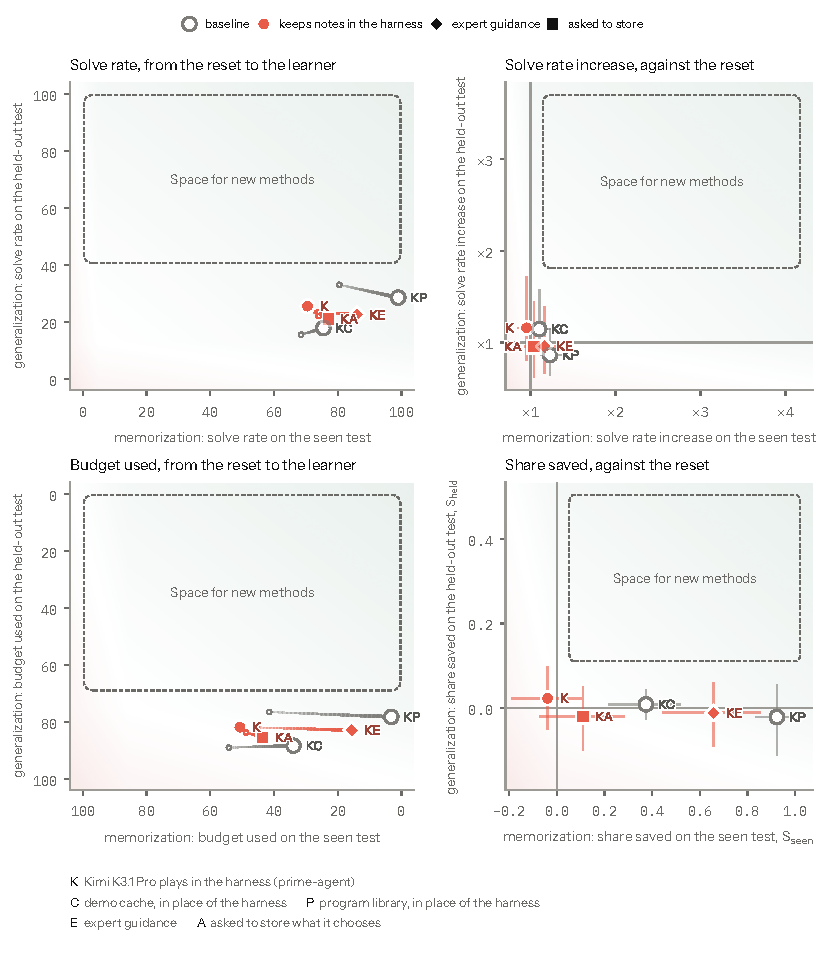
\includegraphics[width=\linewidth]{figures/tests-arc2.pdf}
\caption{Figure~\ref{fig:plane}'s four panels for ARC-AGI-2, with broad axis ranges: every learner Kimi K3.1 Pro has played on this track so far, requested at medium reasoning effort, at one user, each against its reset. The dashed boxes mark the space no learner here reaches yet, which we leave open for new methods and submissions: on the left panels everything above the points drawn, where a learner better on the held-out test than any here would stand, and on the right an open region above and to the right of no gain.}
\label{fig:plane-arc2}
\end{figure}

\begin{figure}[htbp]
\centering
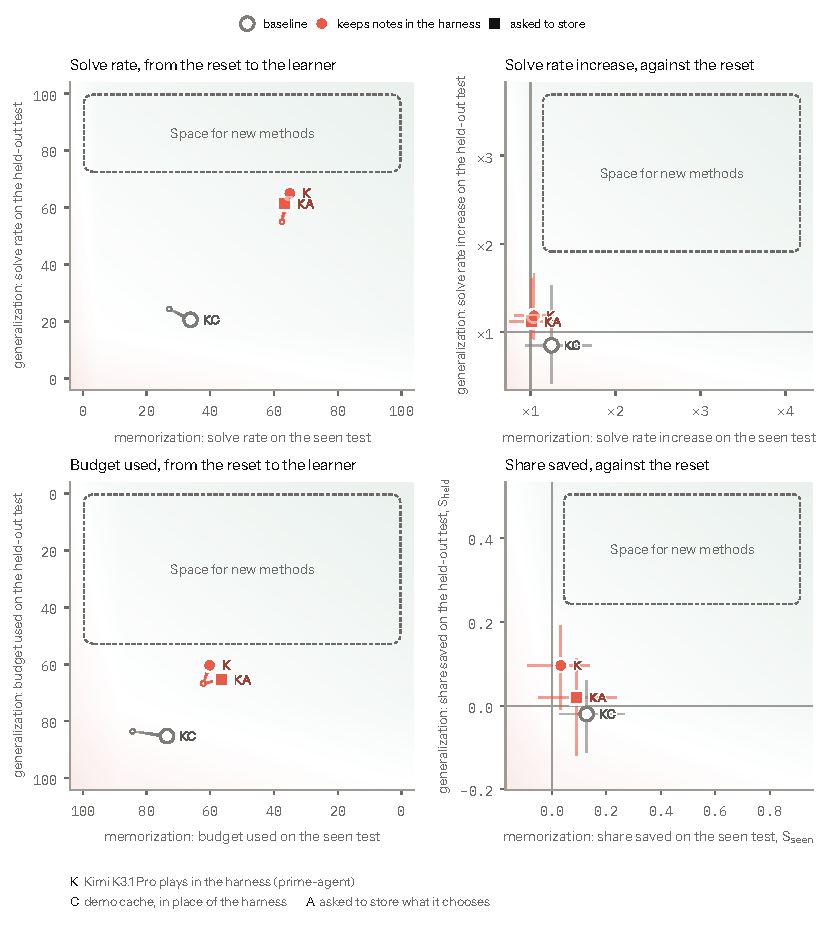
\includegraphics[width=\linewidth]{figures/tests-arc3.pdf}
\caption{Figure~\ref{fig:plane}'s four panels for ARC-AGI-3, as Figure~\ref{fig:plane-arc2} draws them for ARC-AGI-2, with the space left open boxed the same way. The program library and the expert guidance are procedures for grids, so they do not play this track, beyond the pilot of a version of each for games in Appendix~\ref{app:tracks-pilot}, which played no test.}
\label{fig:plane-arc3}
\end{figure}

\paragraph{A pilot of KP and KE on ARC-AGI-3.}
\label{app:tracks-pilot}
On ARC-AGI-3 an answer is a sequence of actions rather than a grid, so we built a version of each procedure for games. The program library keeps a world model per game, a program that gives the board after an action and whether a board is won. It is checked at no cost against every transition the game has shown, the demonstrations' and the learner's own, and kept once it gets none wrong. When the game returns, a fixed search plans the level with the kept program, and the plan is played before the model is asked, stopping at the first board the program did not predict. The expert guidance tells prime-agent to request a demonstration of a new game, try each action it did not show and keep notes on the controls and the win condition. It also tells it to write, check and plan with a world model through the check and the search, given as tools. Each played the stream once, with no test and no wiped twin, and Table~\ref{tab:arc3-pilot} reads them beside the methods of Table~\ref{tab:tracks-light} on the same instances. KE solved the most and spent the least, and on returns it solved 12.4 points more than K [7.6, 18.1] at 1.77 less charge [$-2.44$, $-1.09$], with 95\% intervals over the 15 games. Its first visits gained as much, and its returns solved no more than its first visits, so the gain lies in how it plays a game it meets. What it learned across visits is for its wiped twin to show. It kept notes and trajectories for every game, and no program. KP did no better than the floors. It kept programs for three games, and their plans won sp80's last six visits and ft09's last four with no model call, each for 0.09 to 0.10 of the budget of 8. It lost its first visits, solving 1 of 15 against the demo-cache floor's 6, for a reason we have not shown (\texttt{scripts/read\_arc3\_pilot.py}).

